\documentclass[12pt,twoside]{report}

%%%%%%%%%%%%%%%%%%%%%%%%%%%%%%%%%%%%%%%%%%%%%%%%%%%%%%%%%%%%%%%%%%%%%%%%%%%%%

% Definitions for the title page
% Edit these to provide the correct information
% e.g. \newcommand{\reportauthor}{Timothy Kimber}

\newcommand{\reporttitle}{Analysing property sales data using Data Science}
\newcommand{\reportauthor}{Wenxiang Luo}
\newcommand{\supervisor}{Chiraag Lala}
\newcommand{\degreetype}{MSc Computing}

%%%%%%%%%%%%%%%%%%%%%%%%%%%%%%%%%%%%%%%%%%%%%%%%%%%%%%%%%%%%%%%%%%%%%%%%%%%%%

% load some definitions and default packages
%%%%%%%%%%%%%%%%%%%%%%%%%%%%%%%%%%%%%%%%%
% University Assignment Title Page 
% LaTeX Template
% Version 1.0 (27/12/12)
%
% This template has been downloaded from:
% http://www.LaTeXTemplates.com
%
% Original author:
% WikiBooks (http://en.wikibooks.org/wiki/LaTeX/Title_Creation)
%
% License:
% CC BY-NC-SA 3.0 (http://creativecommons.org/licenses/by-nc-sa/3.0/)
% 
%
%%%%%%%%%%%%%%%%%%%%%%%%%%%%%%%%%%%%%%%%%
%----------------------------------------------------------------------------------------
%	PACKAGES AND OTHER DOCUMENT CONFIGURATIONS
%----------------------------------------------------------------------------------------
\usepackage[a4paper,hmargin=2.8cm,vmargin=2.0cm,includeheadfoot]{geometry}
\usepackage{textpos}
\usepackage[numbers]{natbib} % for bibliography
\usepackage{tabularx,longtable,multirow,subfigure,caption}%hangcaption
\usepackage{fncylab} %formatting of labels
\usepackage{fancyhdr} % page layout
\usepackage{url} % URLs
\usepackage[english]{babel}
\usepackage{amsmath}
\usepackage{graphicx}
\usepackage{dsfont}
\usepackage{epstopdf} % automatically replace .eps with .pdf in graphics
\usepackage{backref} % needed for citations
\usepackage{array}
\usepackage{latexsym}
\usepackage[pdftex,pagebackref,hypertexnames=false,colorlinks]{hyperref} % provide links in pdf

\hypersetup{pdftitle={},
  pdfsubject={}, 
  pdfauthor={},
  pdfkeywords={}, 
  pdfstartview=FitH,
  pdfpagemode={UseOutlines},% None, FullScreen, UseOutlines
  bookmarksnumbered=true, bookmarksopen=true, colorlinks,
    citecolor=black,%
    filecolor=black,%
    linkcolor=blue,%
    urlcolor=black}

\usepackage[all]{hypcap}


%\usepackage{color}
%\usepackage[tight,ugly]{units}
%\usepackage{float}
%\usepackage{tcolorbox}
%\usepackage[colorinlistoftodos]{todonotes}
% \usepackage{ntheorem}
% \theoremstyle{break}
% \newtheorem{lemma}{Lemma}
% \newtheorem{theorem}{Theorem}
% \newtheorem{remark}{Remark}
% \newtheorem{definition}{Definition}
% \newtheorem{proof}{Proof}


%%% Default fonts
\renewcommand*{\rmdefault}{bch}
\renewcommand*{\ttdefault}{cmtt}



%%% Default settings (page layout)
\setlength{\parindent}{0em}  % indentation of paragraph

\setlength{\headheight}{14.5pt}
\pagestyle{fancy}
\renewcommand{\chaptermark}[1]{\markboth{\chaptername\ \thechapter.\ #1}{}} 

\fancyfoot[ER,OL]{\sffamily\textbf{\thepage}}%Page no. in the left on odd pages and on right on even pages
\fancyfoot[OC,EC]{\sffamily }
\renewcommand{\headrulewidth}{0.1pt}
\renewcommand{\footrulewidth}{0.1pt}
\captionsetup{margin=10pt,font=small,labelfont=bf}


%--- chapter heading

\def\@makechapterhead#1{%
  \vspace*{10\p@}%
  {\parindent \z@ \raggedright \sffamily
    \interlinepenalty\@M
    \Huge\bfseries \thechapter \space\space #1\par\nobreak
    \vskip 30\p@
  }}

%---chapter heading for \chapter*  
\def\@makeschapterhead#1{%
  \vspace*{10\p@}%
  {\parindent \z@ \raggedright
    \sffamily
    \interlinepenalty\@M
    \Huge \bfseries  #1\par\nobreak
    \vskip 30\p@
  }}

\allowdisplaybreaks

% load some macros
% Here, you can define your own macros. Some examples are given below.

\newcommand{\R}[0]{\mathds{R}} % real numbers
\newcommand{\Z}[0]{\mathds{Z}} % integers
\newcommand{\N}[0]{\mathds{N}} % natural numbers
\newcommand{\C}[0]{\mathds{C}} % complex numbers
\renewcommand{\vec}[1]{{\boldsymbol{{#1}}}} % vector
\newcommand{\mat}[1]{{\boldsymbol{{#1}}}} % matrix


\date{June 2022}

\begin{document}

% load title page
% Last modification: 2015-08-17 (Marc Deisenroth)
\begin{titlepage}

\newcommand{\HRule}{\rule{\linewidth}{0.5mm}} % Defines a new command for the horizontal lines, change thickness here


%----------------------------------------------------------------------------------------
%	LOGO SECTION
%----------------------------------------------------------------------------------------


\includegraphics[width = 4cm]{./figures/imperial}\\[0.5cm] 

\center % Center remainder of the page

%----------------------------------------------------------------------------------------
%	HEADING SECTIONS
%----------------------------------------------------------------------------------------

\textsc{\Large Imperial College London}\\[0.5cm] 
\textsc{\large Department of Computing}\\[0.5cm] 

%----------------------------------------------------------------------------------------
%	TITLE SECTION
%----------------------------------------------------------------------------------------

\HRule \\[0.4cm]
{ \huge \bfseries \reporttitle}\\ % Title of your document
\HRule \\[1.5cm]
 
%----------------------------------------------------------------------------------------
%	AUTHOR SECTION
%----------------------------------------------------------------------------------------

\begin{minipage}{0.4\textwidth}
\begin{flushleft} \large
\emph{Author:}\\
\reportauthor % Your name
\end{flushleft}
\end{minipage}
~
\begin{minipage}{0.4\textwidth}
\begin{flushright} \large
\emph{Supervisor:} \\
\supervisor % Supervisor's Name
\end{flushright}
\end{minipage}\\[4cm]


%----------------------------------------------------------------------------------------
%	FOOTER & DATE SECTION
%----------------------------------------------------------------------------------------
\vfill % Fill the rest of the page with whitespace
Submitted in partial fulfillment of the requirements for the MSc degree in
\degreetype~of Imperial College London\\[0.5cm]

\makeatletter
\@date 
\makeatother


\end{titlepage}



% page numbering etc.
\pagenumbering{roman}
\clearpage{\pagestyle{empty}\cleardoublepage}
\setcounter{page}{1}
\pagestyle{plain}
\graphicspath{ {./figures/} }

%%%%%%%%%%%%%%%%%%%%%%%%%%%%%%%%%%%%
\begin{abstract}
Your abstract.
\end{abstract}

\cleardoublepage
%%%%%%%%%%%%%%%%%%%%%%%%%%%%%%%%%%%%
\section*{Acknowledgments}
Comment this out if not needed.

\clearpage{\pagestyle{empty}\cleardoublepage}

%%%%%%%%%%%%%%%%%%%%%%%%%%%%%%%%%%%%
%--- table of contents
\fancyhead[RE,LO]{\sffamily {Table of Contents}}
\tableofcontents 


\clearpage{\pagestyle{empty}\cleardoublepage}
\pagenumbering{arabic}
\setcounter{page}{1}
\fancyhead[LE,RO]{\slshape \rightmark}
\fancyhead[LO,RE]{\slshape \leftmark}

%%%%%%%%%%%%%%%%%%%%%%%%%%%%%%%%%%%%
\chapter{Introduction}

Nowadays, there is a substantial amount of data generated every second. The daily lives of humans are producing it, and some other fields, such as research, health care, economic activities, and environmental information from various sensors, also generate a vast amount of data. Obtaining the relationship between some features or the patterns underlying these massive amounts of data might benefit the entire world. For instance, new causes of diseases might be identified, and technological advancement could be accelerated.
\\

However, this extensive data can be one of the main obstacles for analysis as it is approximately impossible for humans to obtain insights into the data manually. Under this circumstance, artificial intelligence (AI), a technique that empowers the computer to imitate human intelligence and manner,  could be one of the methods to mitigate this issue. It can extract patterns from large datasets and use them to make predictions based on future data and even identify which data components are responsible for the results.
\\

In this project, some AI techniques will be applied to property and demographic data to gain insights and understand the factors influencing a homeowner's likelihood to sell. The factors might include the proximity to schools, hospitals, or supermarkets, the accessibility to public transportation, and the property types (flats or houses). It could be highly advantageous to estate agents who would discover homeowners with more potential to become clients and provide them with business. 

\section{Aim \& Objective}
\section{Layout of the Report}

%%%%%%%%%%%%%%%%%%%%%%%%%%%%%%%%%%%%
\chapter{Literal Review}
Python is one of the most popular programming languages in the world since it is simple to develop, and there are extensive packages for various functionalities. In this project, Python and its packages would be used for loading data, preprocessing data, and constructing and evaluating machine learning models. 

\section{Machine Learning}
Machine Learning (ML), a subset of AI, is a technique that the computer can learn and improve from data without explicit programming. The reason for utilizing ML is that its performance is sometimes better than the conventional approach. For example, ML techniques would simplify the solution to a problem that comprises a long list of rules (spam mail detection). 
\\

ML can be divided into three categories, one of which is supervised learning. In supervised learning, the dataset contains features (input to the model) and targets (ground truth of the output), and the model's parameters are randomly initialized. Then the features are passed to the model, and the differences between the current output and the ground truth are used to update the parameters until the differences are acceptable. 
\\

In this project, a supervised learning model will be implemented for data analysis, and the steps are listed below.
\begin{enumerate}
	\item Data Preprocessing: Some data from the dataset may be missing, and these values must be handled appropriately before being passed to the model. 
	\item Standardization: In real life, different features usually have different ranges, and this will cause a problem in ML, which is that high magnitude features would have more weight than low magnitude features \citep{RN4}. One of the solutions is standardization, which could scale all the features to the same magnitude.
	\item Feature encoding: ML models require numerical values, whereas the categorical features in the dataset do not satisfy this requirement. Therefore, these features should be converted into numerical values. 
	\item Training \& Testing: The parameters of the model are updated, and it is expected that the loss will converge during training. The performance of the model is validated when testing.
\end{enumerate}

\section{Handle Text Information}
The format of texts in this project could be classified as HTML and plaintext. Although Python standard libraries provide some string processing capabilities, they are insufficient for this situation. 

\subsection{Beautiful Soup}
\textit{\textbf{Beautiful Soup}} is a Python library for extracting data from markup languages, such as HTML and XML. It can accomplish this with a user-specified parser, for example, \textbf{\textit{html.parser}}, to navigate, search and modify the parse tree, which would save considerable time \citep{RN10}. 

\subsection{parse}
The \textit{\textbf{format}} function in the Python standard library formats a string, whereas the \textit{\textbf{parse}} module provides functions with an oppositse effect, i.e., extract information from formatted strings.

\subsection{Regular Expression}
A regular expression is a sequence of ordinary and special characters representing textual patterns. The ordinary characters are identical throughout the expressions and texts, while the special characters specify the pattern, including number, location, and type of characters  \citep{RN14}. One of the primary disadvantages of the regular expression is its obscure syntax, which results in difficulty specifying a pattern. 

\subsection{Library Usage}
In this project, HTML texts are used extensively in the raw dataset to describe property summaries, property layouts, and council tax. This is the optimal scenario for \textit{Beautiful Soup} which is employed to extract plaintext by specifying tags. Then, \textit{parse} is applied to obtain the information, such as room names, from the plaintexts since they are in the same format. In addition, due to its limitations, the regular expression is only used to acquire numerical values in this project. 


\section{Data Manipulation}
\subsection{NumPy}
Numerical Python (\textit{\textbf{NumPy}}) is a scientific computing package that was designed to support large multidimensional matrices. It uses an optimized \textit{C/C++} API to reduce computation time compared to pure Python computations \citep{RN6}. A substantial number of complex tasks of data analytics can be simplified by numerous \textit{numpy} features. For example, it provides robust matrix operations, facilitates the construction of multidimensional objects, and serves as the fundation of other packages, including \textit{matplotlib} and \textit{seaborn}.

\subsection{Pandas}
The \textbf{\textit{pandas}} is an open-source and compelling package that was developed primarily for data analysis and data manipulation and is built on \textit{numpy}. It is capable of handling data of various types (numerical values, strings, and time) and from a variety of sources (CSV, Excel, and MqSQL database). \textbf{\textit{DataFrame}} is one of the \textit{pandas} data structures that is appropriate for handling tabular data with columns of different types. Additionally, it could manage various operations, such as manipulating missing values, creating pivot tables, and grouping data from different columns \citep{RN4}. 

\subsection{Library Usage}
In this project, the dataset provided is in CSV format hence it could be loaded by \textbf{\textit{Pandas}} since it is suitable for tabular data. Then the package is utilized for preprocessing, such as handling missing values and grouping columns of data. 
\\

\textit{\textbf{Numpy}} is appropriate for manipulating numerical data and acts as an intermediary between various packages. Therefore, it could be employed to evaluate the performance of ML models and transmit data to plotting packages. 


\section{ML Frameworks}
\subsection{Scikit-learn}
\textit{\textbf{Scikit-learn}} is a popular open-source ML framework that employs \textit{Numpy}. It contains traditional ML algorithms, including clustering, classification, and regression, as well as a variety of utilities that can be applied to preprocess data and evaluate the performance \citep{RN7}. The drawback of this library is that it does not natively support GPU acceleration and is not a neural network framework. 

\subsection{PyTorch}
\textbf{\textit{PyTorch}} is one of the popular ML frameworks developed by Facebook, which is designed to implement neural networks with flexibility and speed \citep{RN5}. It provides various components for model construction and training. For instance, there are numerous types of modules that comprise a model, such as linear layers, dropout, and activation functions, as well as a variety of loss functions and optimizers that can be employed in model training. 
\\

Furthermore, it can be beneficial to construct and train a model with \textit{Pytorch}. It has a Pythonic nature which means that its syntax is similar to Python, making it more straightforward for Python programmers to develop neural networks than other ML frameworks. Moreover, it is a rapidly expanding framework for developing neural networks with a vast ecosystem, meaning that a substantial number of utilities have been developed on top of it \citep{RN5}. Additionally, \textit{PyTorch} supports automatic differentiation and GPU acceleration which can be advantageous for model training.

\subsection{TensorFlow}
\textit{\textbf{TensorFlow}} is another ML framework produced by Google that specializes in deep learning and neural networks. It provides approximately the same components as \textit{PyTorch} and also supports automatic differentiation and GPU acceleration. One of the appealing characteristics of \textit{TensorFlow} is called \textit{\textbf{TensorBoard}}, which is an interactive visualization system that can display the flowchart of the data manipulation and plot the tendency of the performance \citep{RN15}. 

\subsection{Library Usage}
This project aims to construct a neural network which means \textit{scikit-learn} is not applicable at this stage. Although \textit{TensorFlow} provides the same capabilities as \textit{PyTorch} and is superior in visualization, the model construction and training will use \textit{PyTorch} due to its Pythonic syntax and compatibility with \textit{TensorBoard}. 
\\

However, \textit{scikit-learn} can be used to preprocess datasets and evaluate performance. It provides various utilities that can be helpful before training, for example, encoding categorical features and splitting the dataset into training and validation. In addition, it offers features for model evaluation, such as confusion matrix, accuracy, and recall. 

\section{Data Visualization}
\subsection{Matplotlib \& Seaborn}
\textbf{\textit{Matplotlib}} is a Python package for 2D plotting that produces high-quality figures. It supports both interactive and non-interactive plotting and can save images in multiple formats, including PNG and JPEG. It can also generate numerous types of graphs, such as line plots, scatter plots, and pie plots.

\subsection{Seaborn}
\textbf{\textit{Seaborn}} is a Python library for creating statistical graphs that integrates with \textit{pandas} to offer a high-level interface to \textit{matploblib}. If a dataset is provided, \textit{seaborn} can automatically generate the figure with appropriate plotting attributes, such as color and legend. Additionally, it is capable of generating comprehensive graphics with a single function call and a minimum number of arguments \citep{RN16}.

\subsection{Library Usage}


\section{Methodology}

%%%%%%%%%%%%%%%%%%%%%%%%%%%%%%%%%%%%
\chapter{Implementation}
\section{Data Preprocessing}
The data that was retrieved for this project originated from two different sources: a raw dataset and online APIs. 

\subsection{Extract Values}
There are two types of data in the raw dataset: HTML texts containing the property information and categorical keywords describing features, such as parking spaces and heating.

\subsubsection{Handle Room Descriptions (HTML)}
\textbf{\textit{\underline{Acquire room name and dimension}}} \\
The structure of the HTML texts containing the room information in a property is shown in figure \ref{html_structure}. The rooms are separated by tag \textit{$<$li$>$}, and the room name and its dimension is denoted by \textit{$<$strong$>$} and \textit{$<$i$>$} tags, respectively. Therefore, a function (\textit{\textbf{EweMove\_Description\_S3\_Rooms}}) was implemented to split the HTML text by utilizing \textit{Beautiful soup}, and its flowchart is shown in figure \ref{html_room_info}.
\begin{figure}[h]
	\centering
	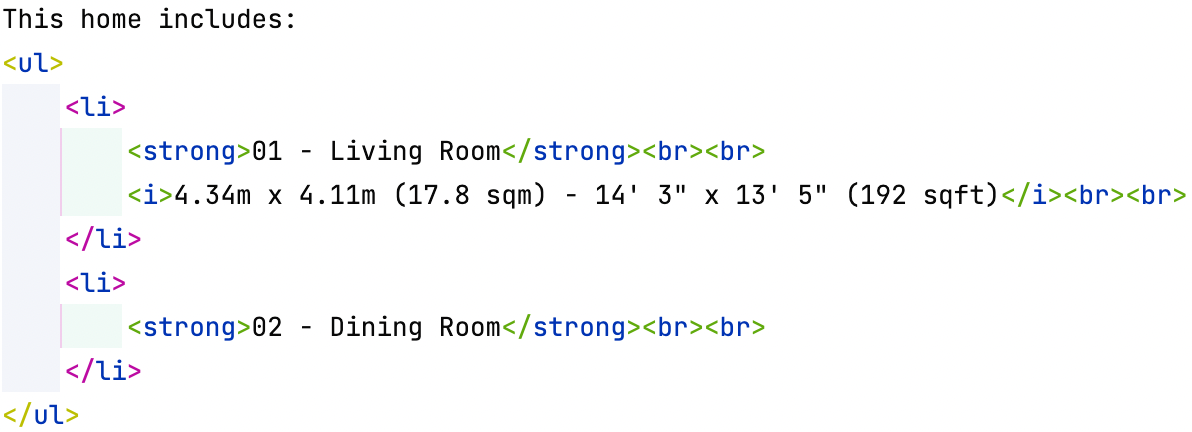
\includegraphics[width=15cm]{html_structure}
	\caption{The layout of HTML texts}
	\label{html_structure}
\end{figure}

\begin{figure}[h]
	\centering
	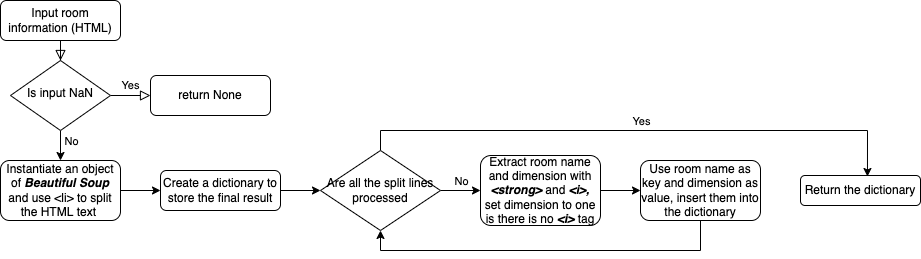
\includegraphics[width=15cm]{html_room_info}
	\caption{Flowchart for extracting room information from HTML}
	\label{html_room_info}
\end{figure}

The names of rooms are analyzed after the room descriptions in the dataset have been processed. As a consequence, there are over 200 unique room names for approximately 3600 records, some of which are exceptionally uncommon across the entire dataset. For instance, only two properties have cinema rooms and one has a lift, which is less than 0.1\% of all entries.  
\\

Due to the large number of room names, it is impossible to use it as the input of the model. Therefore, the rooms are divided into seven categories: bedrooms, bathrooms, kitchens, living/reception rooms, dining rooms, work areas, and other rooms so that the data can be generalized. 
\\

\textbf{\textit{\underline{Generalize room information}}} \\
A class, \textit{\textbf{ExtractRooms}}, was developed to acquire and integrate the room information, especially the area in square meters, and its UML diagram is shown in figure \ref{uml_extract_rooms}. The member variable \textit{rooms} is a list containing the result of invoking \textit{EweMove\_Description\_S3\_Rooms}, \textit{room\_set} comprises all the room names, \textit{current\_rooms} consists of the room names that have been processed, and \textit{extract\_area} is a formatted string for acquiring room area. 
\\

\begin{figure}[h]
	\centering
	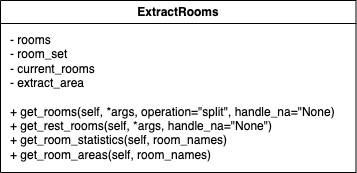
\includegraphics[width=10cm]{uml_extract_rooms}
	\caption{The UML diagram of the class (\textit{ExtractRooms})}
	\label{uml_extract_rooms}
\end{figure}

Key member functions
\begin{itemize}
	\item get\_rooms \\
	The flow diagram of this method is shown in figure \ref{extract_room_get_rooms} and the arguments are listed below.
	\begin{enumerate}
		\item args: It should be noted that this is a variable-length argument, which means that it can accept as many arguments as possible, and it is used to select room names from \textit{room\_set}. For instance, \textit{*args = ["living", "reception"]} will select all names containing "living" or "reception". 
		\item operation: The argumen determines the types of the final result and the valid inputs include \textit{"sum"}, \textit{"mean"}, \textit{"split"}, and \textit{"number"}. For example, if args is "bedroom", then the function can return the sum of bedroom areas, the average bedroom area, the area of each bedroom and the number of bedrooms. 
		\item handle\_na: This parameter specifies how to manage missing values, either by ignoring them or by filling the mean value if the input is "None" or "mean", respectively. 
	\end{enumerate} 
	\begin{figure}[h]
		\centering
		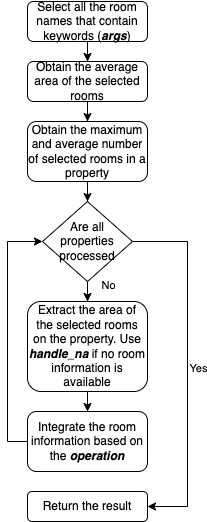
\includegraphics[height=11cm]{extract_room_get_rooms}
		\caption{Flowchart of \textit{get\_rooms}}
		\label{extract_room_get_rooms}
	\end{figure}
	\item get\_rest\_room: \\
	This method is identical to \textit{\textbf{get\_room}} with two exceptions. The parameter \textit{\textbf{*args}} is used to disgard the room names containing the keywords, and only the number and the total areas of other rooms are returned. 
\end{itemize}

\subsection{Manipulate Categorical Keywords}
In the dataset, four features are characterized by categorical keywords, including parking, heating, accessibility, and outdoor spaces. Figure \ref{parking_dataset} is a snippet of the parking dataset that is used as an example to demonstrate the manipulation of the keywords. The first three rows indicate that there is one parking space for the first property, which is allocated off-street parking for residents, the second row has none, and the third property has one on-street parking space.
\begin{figure}[h]
	\centering
	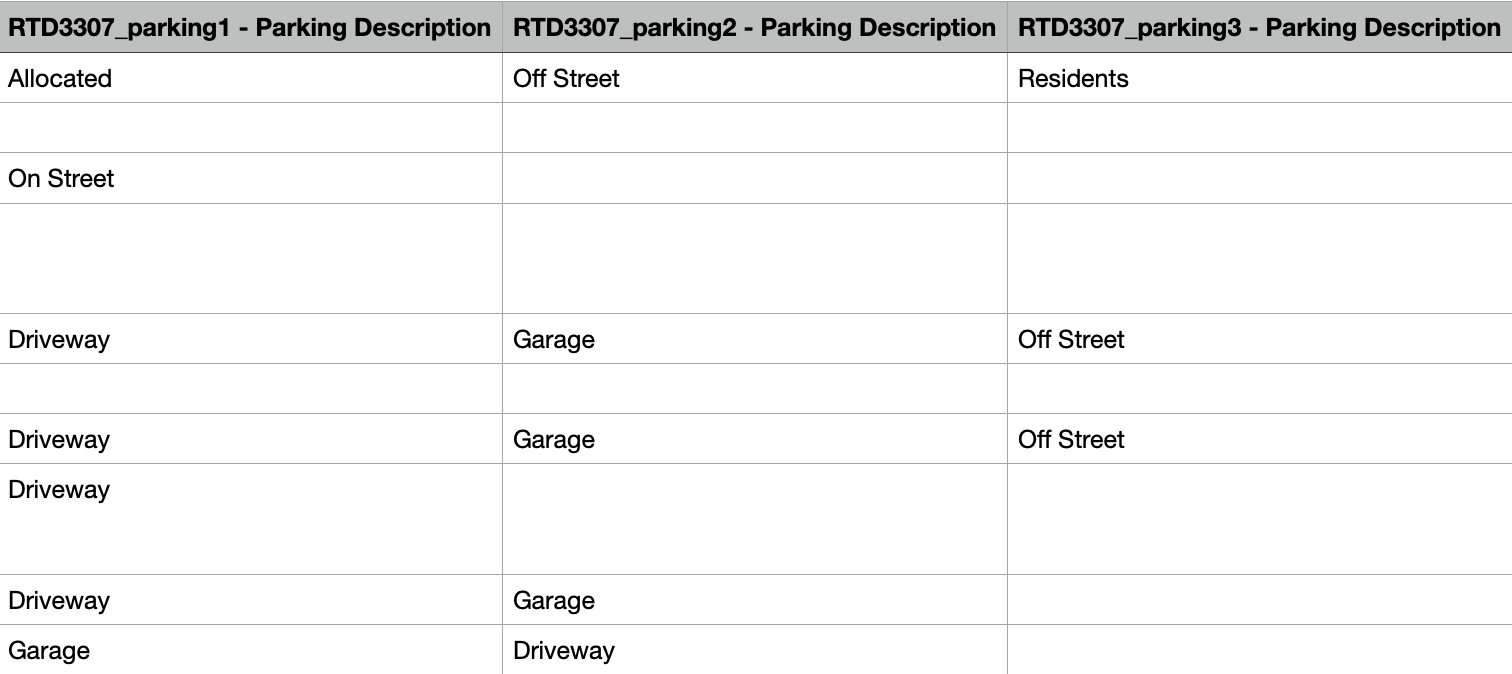
\includegraphics[width=15cm]{parking_dataset}
	\caption{The parking spaces in the first five properties}
	\label{parking_dataset}
\end{figure}

Figure \ref{uml_generalize_dataset} illustrates the UML diagram of the class \textit{\textbf{GeneralizeDataset}}, which was developed to determine how these features of each property are described and the number of keywords within the description. The core of this class is member function \textit{\textbf{get\_feature\_types}}, and its flowchart is displayed in figure \ref{generalize_dataset_get_feature_types}. In addition, function \textbf{\textit{get\_feature\_num}} can be used to determine the number of keywords for each property. 
\begin{figure}[h]
	\centering
	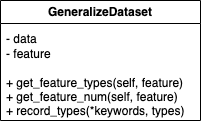
\includegraphics[width=5cm]{uml_generalize_dataset}
	\caption{The UML diagram of \textit{GeneralizeDataset}}
	\label{uml_generalize_dataset}
\end{figure}

\begin{figure}[h]
	\centering
	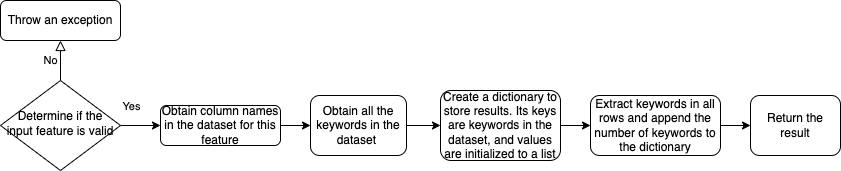
\includegraphics[width=15cm]{generalize_dataset_get_feature_types}
	\caption{Flowchart of \textit{get\_feature\_types}}
	\label{generalize_dataset_get_feature_types}
\end{figure}

%%%%%%%%%%%%%%%%%%%%%%%%%%%%%%%%%%%%
\chapter{Testing the Implementation}
Comprehensive testing was conducted throughout the implementation but it is documented in this separate chapter for the sake of illuatration. 

\section{Data Preprocessing}

\subsection{Extract Values}

\subsubsection{Obtaining Room Information}
There were two tests for this objective, the first test examing if the room name and its dimension can be acquiare from HTML texts and the second test focuses on whether the room areas can be obtained and integrated correctly. 
\\

\textbf{\textit{\underline{Acquire room name and dimension}}} \\
This test utilized two HTML texts, which are illustrated in figure \ref{html_room_info_test}. By invoking the function \textit{\textbf{EweMove\_Description\_S3\_Rooms}} with two snippets, it can be verified that all the room names and dimensions can be extracted without error, and if the dimension is unavailable, it is set to one. 
\\
\begin{figure*}[h]
	\centering
	\subfigure[Snippte 1]{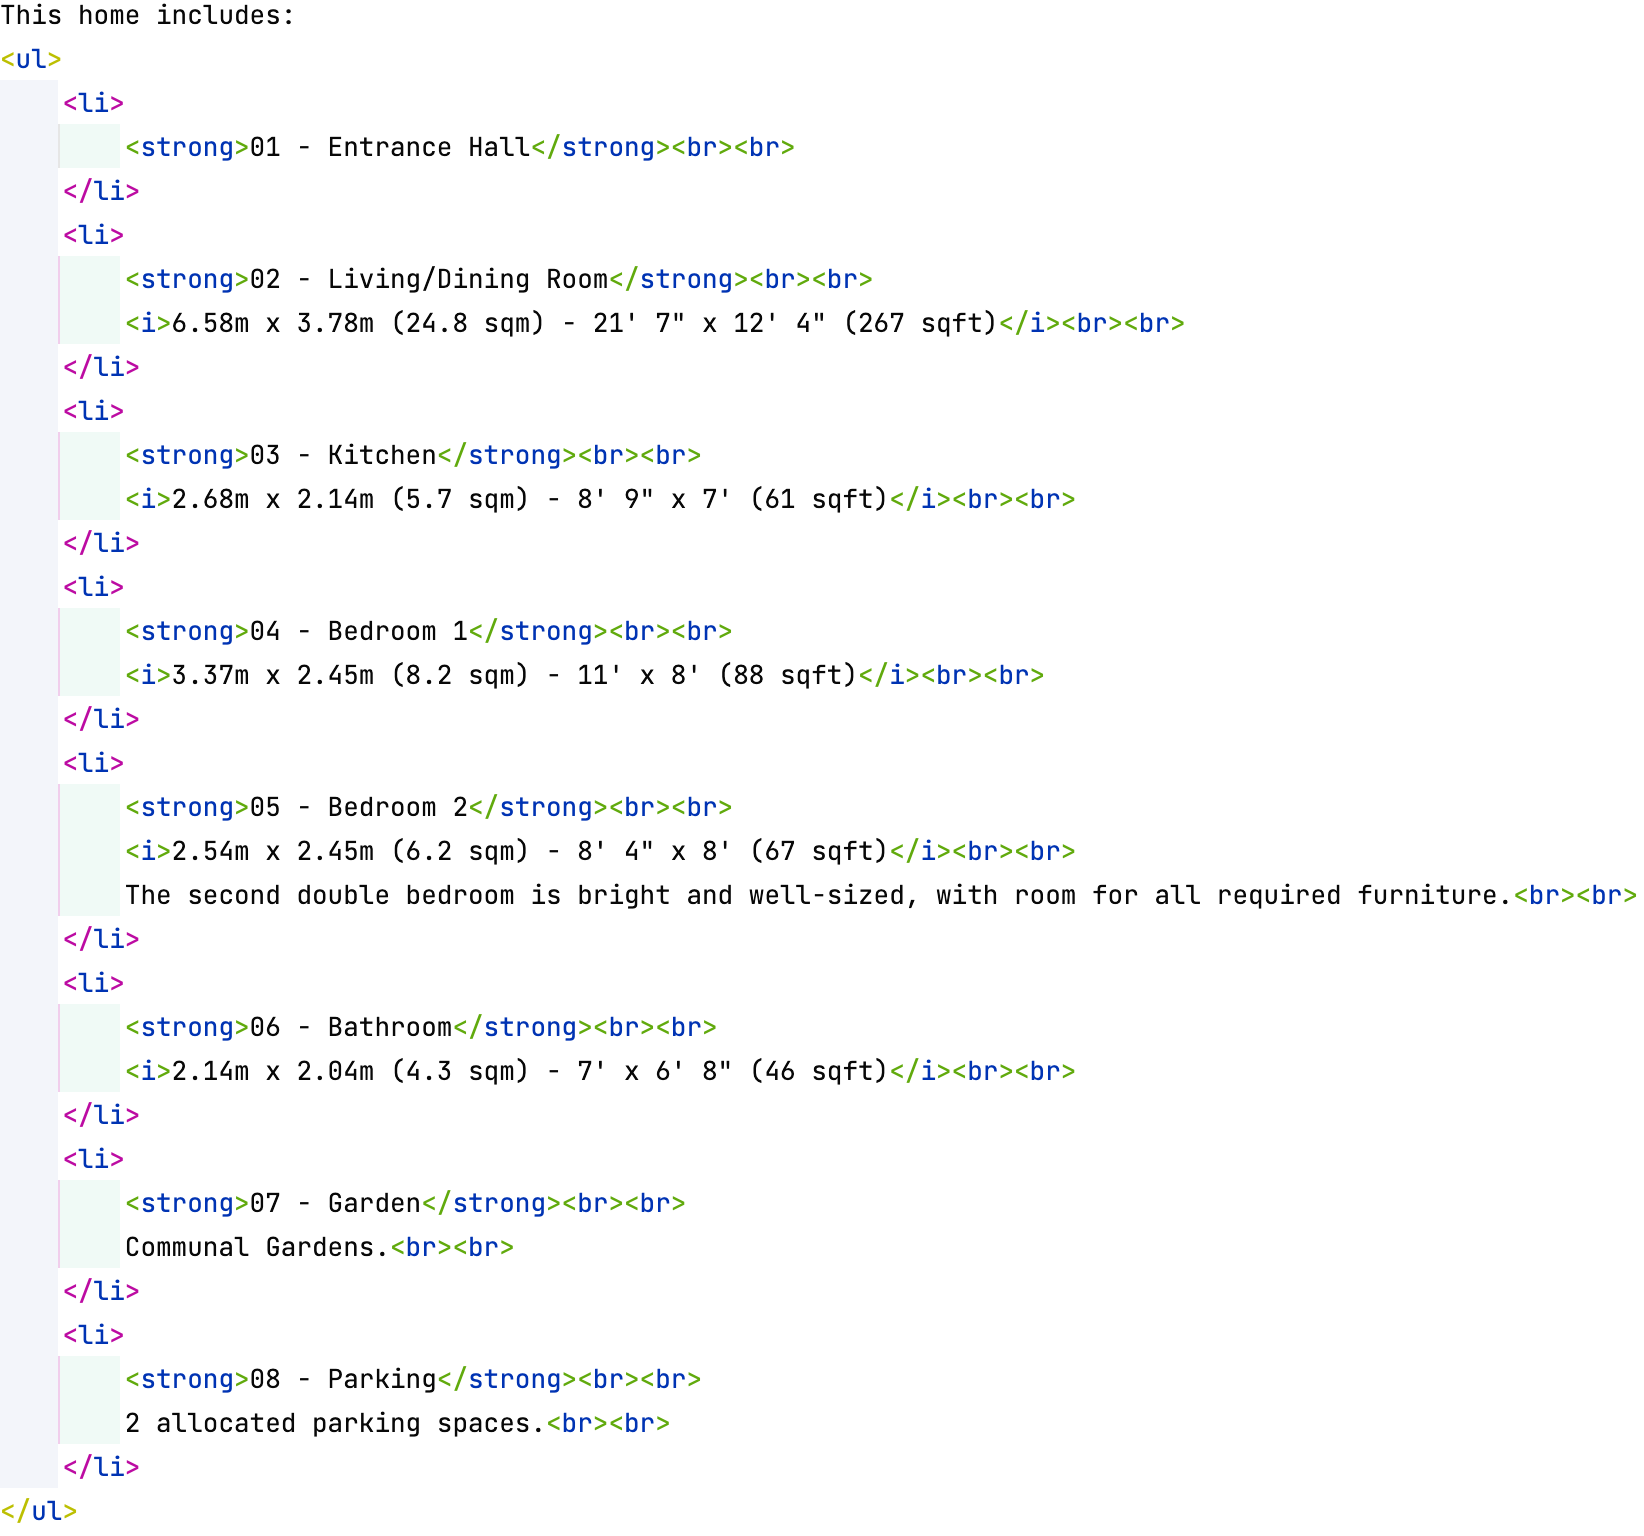
\includegraphics[width=7.5cm, height=8cm]{html_room_info_1}\label{html_room_info_test_1}}
	\hfill
	\subfigure[Snippet 2]{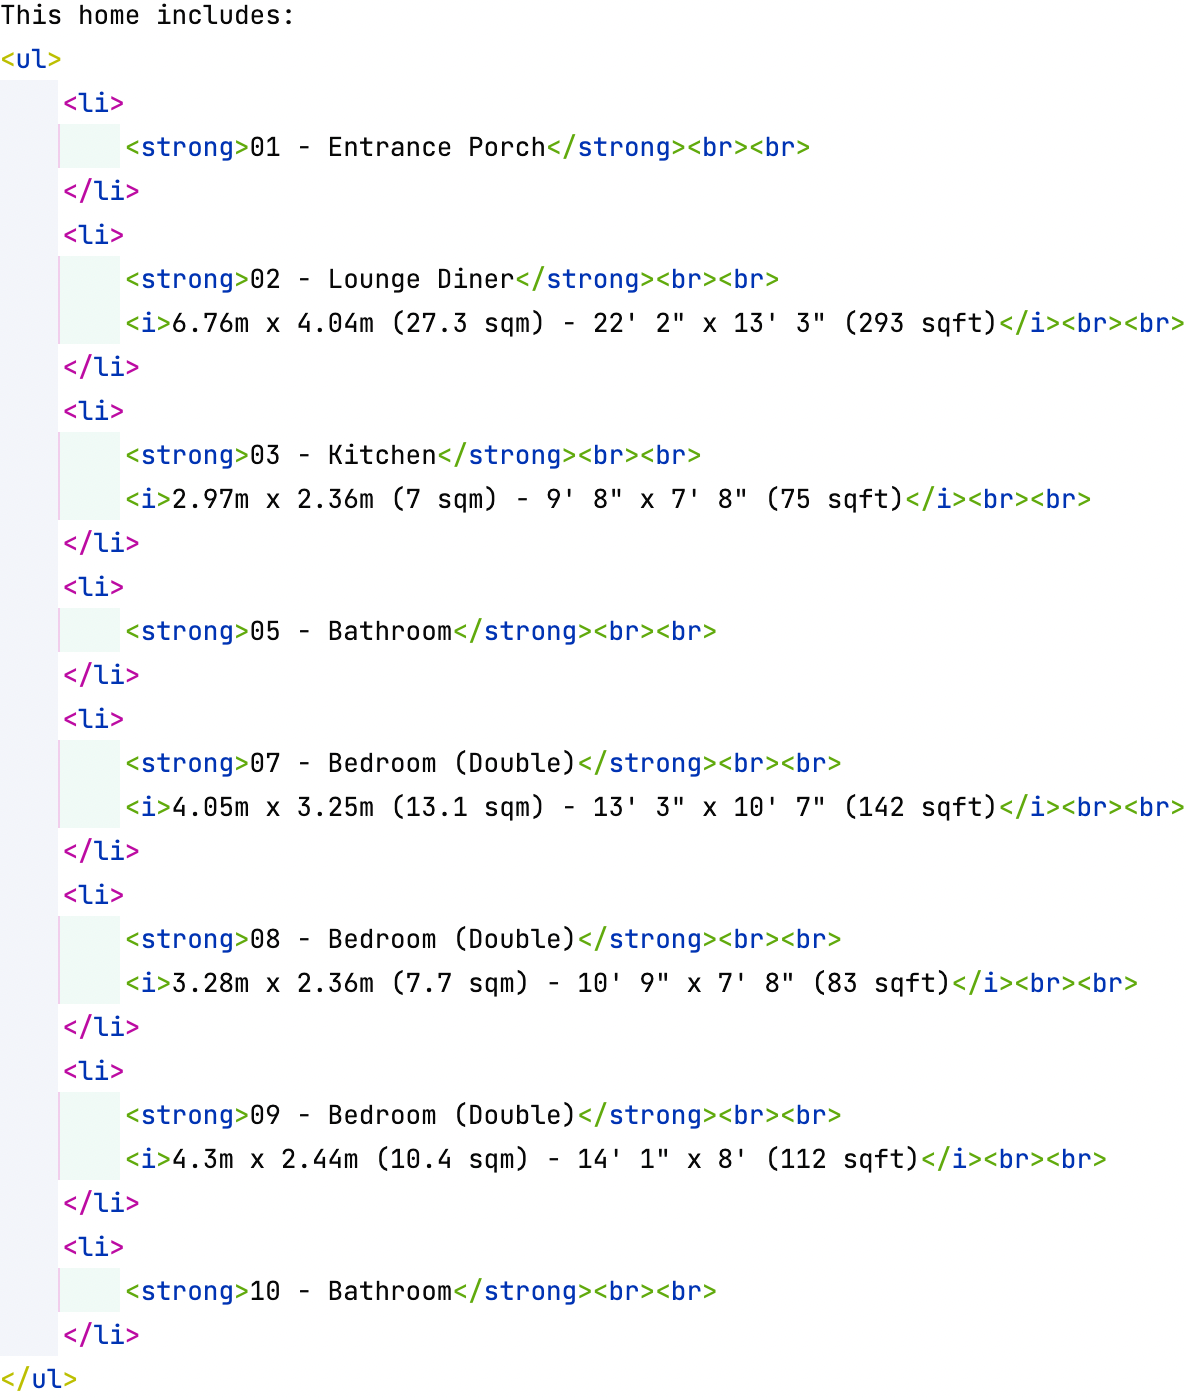
\includegraphics[width=7.5cm, height=8cm]{html_room_info_2}\label{html_room_info_test_2}}
	\caption{The HTML snippets for testing}
	\label{html_room_info_test}
\end{figure*}

\textbf{\textit{\underline{Generalize room information}}} \\
The information obtained from HTML texts (figure \ref{html_room_info_test}) was used to access the behavior of \textit{ExtractRooms}, especially its member functions, \textit{get\_rooms}. During testing, the selected type is the bedroom, and all the operations of \textit{get\_room} were inspected. Additionally, the other rooms were used to test \textit{get\_rest\_rooms}. 
\\

It is guaranteed that if the operation is  "split", then all the bedroom areas can be listed; the sum and average of areas as well as the number of bedrooms will be returned if the function is invoked with corresponding parameters. In addition, the number of other rooms and their total area will be computed correctly. 

\subsection{Manipulate Categorical Keywords}
The data utilized for this test is displayed in figure \ref{parking_dataset}. Initially, an invalid feature, "Distance to School" was input into function \textit{get\_feature\_types}, and it can be assured that an exception would be thrown. The feature was then set to "parking", and the result should be a table with ten rows and six columns, as there are ten properties in the snippet and six keywords in total. In addition, it could be verified that \textit{get\_feature\_num} will return the number of keywords for each property when invoked.

%%%%%%%%%%%%%%%%%%%%%%%%%%%%%%%%%%%%
\chapter{Experimental Results}

\section{Data Preprocessing}

\subsection{Extract Values}

\subsubsection{Obtaining Room Information}
\textbf{\textit{\underline{Acquire room name and dimension}}} \\
After calling the function and retrieving the results (shown in tables \ref{html_room_info_expect_1} and \ref{html_room_info_expect_2}), it is evident that the room names in two HTML snippets could be obtained, and the dimensions were acquired if available otherwise, the value was set to one, hence this function can pass the test.
\begin{table}[h]
	\centering
	\caption{Information from HTML snippet in figure \ref{html_room_info_test_1}}
	\begin{tabular} {| l | l |}
		\hline
		Entrance Hall & 1\\
		\hline
		Living/Dining Room & 6.58m x 3.78m (24.8 sqm) - 21' 7" x 12' 4" (267 sqft)\\
		\hline
		Kitchen & 2.68m x 2.14m (5.7 sqm) - 8' 9" x 7' (61 sqft)\\
		\hline
		Bedroom 1 & 3.37m x 2.45m (8.2 sqm) - 11' x 8' (88 sqft)\\
		\hline
		Bedroom 2 & 2.54m x 2.45m (6.2 sqm) - 8' 4" x 8' (67 sqft)\\
		\hline 
		Bathroom & 2.14m x 2.04m (4.3 sqm) - 7' x 6' 8" (46 sqft)\\
		\hline
		Garden & 1\\
		\hline
		Parking & 1\\
		\hline
	\end{tabular}
	\label{html_room_info_expect_1}
\end{table}

\begin{table}[h]
	\centering
	\caption{Information from HTML snippet in figure \ref*{html_room_info_test_2}}
	\begin{tabular} {| l | l |}
		\hline
		Entrance Porch & 1\\
		\hline
		Lounge Diner & 6.76m x 4.04m (27.3 sqm) - 22' 2" x 13' 3" (293 sqft)\\
		\hline
		Kitchen & 2.97m x 2.36m (7 sqm) - 9' 8" x 7' 8" (75 sqft)\\
		\hline
		Bathroom & 1\\
		\hline
		Bedroom (Double) & 4.05m x 3.25m (13.1 sqm) - 13' 3" x 10' 7" (142 sqft)\\
		\hline 
		Badroom (Double) & 3.28m x 2.36m (7.7 sqm) - 10' 9" x 7' 8" (83 sqft)\\
		\hline
		Bedroom (Double) & 4.3m x 2.44m (10.4 sqm) - 14' 1" x 8' (112 sqft)\\
		\hline
		Bathroom & 1\\
		\hline
	\end{tabular}
	\label{html_room_info_expect_2}
\end{table}

\textbf{\textit{\underline{Generalize room information}}} \\
The results of calling \textit{get\_rooms} are displayed in tables \ref{bedroom_info_split} and \ref{bedroom_info_all}. It is obvious that all the bedrooms and their areas in tables \ref{html_room_info_expect_1} and \ref{html_room_info_expect_2} were successfully extracted. In addition, the numerical values could also be obtained without error if the operations were configured appropriately. These behaviors demonstrated that the functionality and the design are identical. 
\\

Furthermore, the result of invoking \textit{get\_rest\_rooms} is shown in table \ref{other_room_info}. It is clear that there is no statistical inconsistency using the information from tables \ref{bedroom_info_split}, \ref{html_room_info_expect_1}, and \ref{html_room_info_expect_2}, hence this function can pass the test. 
\\ 

In conclusion, the performance of the two crucial member functions in class \textit{ExtractRooms} meets expectations.
\\

\begin{table}[h]
	\centering
	\captionof{table}{Room information ("split")}
	\label{bedroom_info_split}
	\begin{tabular}{| c | c | c | c |}
		\hline
		& Bedroom 1 & Bedroom 2 & Bedroom 3 \\
		\hline
		0 & 8.2 & 6.2 & 0.0 \\
		\hline
		1 & 13.1 & 7.7 & 10.4 \\
		\hline
	\end{tabular}
\end{table}

\begin{table*}[h]
	\centering
	\caption{Bedroom information integrated by different operations}
	\label{bedroom_info_all}
	\subtable[Mean]{
		\begin{tabular}{| c | c |}
			\hline
			& Average area \\ 
			\hline
			0 & 7.2 \\
			\hline
			1 & 10.4 \\ 
			\hline
		\end{tabular}
		\label{bedroom_info_mean}
	}
	\hfill
	\subtable[Sum]{
		\begin{tabular}{| c | c |}
			\hline
			& Total area \\ 
			\hline
			0 & 14.4 \\
			\hline
			1 & 31.2 \\ 
			\hline
		\end{tabular}
		\label{bedroom_info_sum}
	}
	\hfill
	\subtable[Number]{
		\begin{tabular}{| c | c |}
			\hline
			& Number of rooms \\ 
			\hline
			0 & 2 \\
			\hline
			1 & 3 \\ 
			\hline
		\end{tabular}
		\label{bedroom_info_number}
	}
\end{table*}

\begin{table}[h]
	\centering
	\caption{The number and total area of other rooms}
	\label{other_room_info}
	\begin{tabular}{| c | c | c |}
		\hline
		 & Number & Area \\
		 \hline
		 0 & 6 & 34.8 \\
		 \hline
		 1 & 5 & 34.3 \\
		 \hline
	\end{tabular}
\end{table}

\subsection{Manipulate Categorical Keywords}
For the initial test, an exception was thrown if an invalid feature, in this case "Distance to School", was entered. Next, the result of calling function \textit{get\_feature\_types} is shown in table \ref{parking_types}. Apparently, the shape of the table is correct, and its elements are consistent with the dataset snippet. For the first property with an \textbf{allocated} \textbf{off-street} parking space for \textbf{residents}, the three keywords in the first row are set to one while the others are zero, and this conclusion holds true for the remaining properties. In addition, the number of keywords associated with each property can be obtained accurately by calling \textit{get\_feature\_num}. 
\\

In summary,  the member functions in this class are capable to determine the types and number of keywords, hence the implementation can pass the tests.

\begin{table}[h]
	\centering
	\caption{The keywords for each property}
	\label{parking_types}
	\begin{tabular}{| c | c | c | c | c | c | c |}
		\hline
		& Allocated & Driveway & Garage & Off Street & On Street & Residents\\
		\hline
		0 & 1 & 0 & 0 & 1 & 0 & 1 \\ 
		\hline
		1 & 0 & 0 & 0 & 0 & 0 & 0 \\
		\hline
		2 & 0 & 0 & 0 & 0 & 1 & 0 \\
		\hline
		3 & 0 & 0 & 0 & 0 & 0 & 0 \\
		\hline
		4 & 0 & 1 & 1 & 1 & 0 & 0 \\
		\hline
		5 & 0 & 0 & 0 & 0 & 0 & 0 \\
		\hline
		6 & 0 & 1 & 1 & 1 & 0 & 0 \\
		\hline
		7 & 0 & 1 & 0 & 0 & 0 & 0 \\
		\hline
		8 & 0 & 1 & 1 & 0 & 0 & 0 \\
		\hline
		9 & 0 & 1 & 1 & 0 & 0 & 0 \\
		\hline
	\end{tabular}
\end{table}


%%%%%%%%%%%%%%%%%%%%%%%%%%%%%%%%%%%%
\chapter{Conclusion}


%% bibliography
\bibliographystyle{apalike}
\bibliography{proposal}

\end{document}
